\documentclass[11pt,a4paper]{article}

\usepackage[utf8]{inputenc}
\usepackage[T1]{fontenc}
\usepackage{lmodern}
\usepackage[a4paper,margin=2.5cm]{geometry}
\usepackage{graphicx}
\usepackage{amsmath,amssymb}
\usepackage{booktabs}
\usepackage{caption}
\usepackage{subcaption}
\usepackage{float}
\usepackage[hidelinks]{hyperref}
\usepackage{fancyhdr}
\usepackage{xcolor}

\graphicspath{{../results/}}
\captionsetup{font=small,labelfont=bf}

\pagestyle{fancy}
\fancyhf{}
\lhead{\small Computer Methods in Combustion}
\rhead{\small MKWS 2026}
\cfoot{\thepage}
\renewcommand{\headrulewidth}{0.4pt}

\title{\vspace{-1.0cm}\textbf{Effect of Exhaust Gas Recirculation and Oxy-Fuel
Dilution on Methane Combustion}\\[0.3cm]
\large Adiabatic Flame Temperature, Laminar Flame Speed, Auto-Ignition Delay
and NO\textsubscript{x} Formation}

\author{\textbf{Adam Szymianiec} \quad (index no.\ 333507)\\[0.25cm]
Course project --- \emph{Metody Komputerowe w Spalaniu} (MKWS)\\
Warsaw University of Technology, Faculty of Power and Aeronautical Engineering}
\date{June 2026}

\begin{document}
\maketitle
\thispagestyle{fancy}

\begin{abstract}
\noindent This project investigates how two carbon-management combustion
strategies --- \emph{exhaust gas recirculation} (EGR) and \emph{oxy-fuel}
operation --- reshape the combustion of methane relative to a conventional
methane/air baseline. Four complementary quantities are computed with the open
source kinetics library \textsc{Cantera} and the GRI-Mech~3.0 reaction
mechanism: the adiabatic flame temperature (constant-enthalpy equilibrium), the
laminar flame speed (one-dimensional freely-propagating flame), the
auto-ignition delay (zero-dimensional constant-pressure reactor) and the
equilibrium NO concentration. The results quantify the well-known trade-off
behind low-emission combustor design: both EGR and CO\textsubscript{2}-diluted
oxy-fuel combustion lower the flame temperature, slow the flame and lengthen the
ignition delay, but in exchange they suppress thermal NO by up to an order of
magnitude --- and oxy-fuel combustion, by eliminating atmospheric nitrogen,
removes thermal NO almost entirely while yielding a CO\textsubscript{2}-rich
exhaust suited to carbon capture.
\end{abstract}

\section{Introduction}
Stationary gas turbines and reciprocating engines burning natural gas are under
growing pressure to cut both nitrogen-oxide (NO\textsubscript{x}) emissions and
the carbon-capture penalty of their exhaust. Two strategies dominate the
discussion. In \textbf{exhaust gas recirculation} (EGR) a fraction of the cooled
burned gas is re-inducted with the fresh charge; the additional
CO\textsubscript{2} and H\textsubscript{2}O act as a thermal ballast that lowers
the peak temperature and, through the strong temperature sensitivity of the
Zeldovich mechanism, throttles thermal NO. In \textbf{oxy-fuel} combustion the
nitrogen of air is replaced by recycled CO\textsubscript{2}, so the fuel burns
in an O\textsubscript{2}/CO\textsubscript{2} atmosphere; this both removes the
nitrogen that feeds thermal NO and produces an exhaust that is essentially
CO\textsubscript{2} and water vapour, from which CO\textsubscript{2} can be
separated by simple condensation.

Both strategies, however, degrade combustion: a colder flame is slower, harder
to ignite and more prone to instability. The purpose of this project is to make
that trade-off quantitative for methane, the principal constituent of natural
gas, using a single consistent chemical mechanism so that the temperature,
flame-speed, ignition and emission effects can be compared on equal footing.

\section{Literature review}
The adiabatic flame temperature and equilibrium composition of hydrocarbon/air
mixtures are classical results of chemical thermodynamics and are reproduced
here only as a baseline. The laminar burning velocity of stoichiometric
methane/air at ambient conditions is firmly established at
0.36--0.40 m/s both experimentally and with detailed
mechanisms such as GRI-Mech~3.0, and peaks slightly rich, near
$\phi \approx 1.05$--$1.10$. The temperature dependence of methane
auto-ignition follows Arrhenius behaviour with an apparent activation energy of
roughly $2\times10^{5}$ J/mol, spanning several orders of magnitude across
the 1000--1800 K window relevant to engines.

The suppression of thermal NO by flue-gas dilution is the physical basis of
practically every low-NO\textsubscript{x} gas-turbine combustor, and oxy-fuel
combustion with flue-gas recirculation is a leading candidate for
carbon-capture-ready power generation. The replacement of N\textsubscript{2} by
CO\textsubscript{2} is known to reduce the burning velocity markedly, because
CO\textsubscript{2} has a substantially higher molar heat capacity than
N\textsubscript{2} and because it participates chemically through
CO\textsubscript{2} + H $\rightleftharpoons$ CO + OH, which competes with the
chain-branching pool. The present study reproduces these established trends and
collects them into a single comparative framework.

\section{Numerical model}
\subsection{Software and chemistry}
All computations use \textsc{Cantera}~3.2 with the GRI-Mech~3.0 mechanism
(53 species, 325 reactions), which was developed and validated for natural-gas
combustion and includes the nitrogen sub-mechanism required for NO. Unless
stated otherwise the unburned/reference state is
$T_u = 300 K$ and $p = 1 atm$.

\subsection{Mixture definitions}
The fuel is methane and the stoichiometric reference is
$\mathrm{CH_4 + 2\,(O_2 + 3.76\,N_2)}$. The equivalence ratio $\phi$ scales the
fuel relative to this stoichiometric oxidiser. Three families of fresh charge
are studied:
\begin{itemize}
  \item \textbf{Air} --- CH\textsubscript{4} with air
  (O\textsubscript{2}:N\textsubscript{2} = 1:3.76).
  \item \textbf{Oxy-fuel} --- the oxidiser is an
  O\textsubscript{2}/CO\textsubscript{2} blend with a prescribed
  O\textsubscript{2} mole fraction $x_{\mathrm{O_2}}$;
  $x_{\mathrm{O_2}} = 0.21$ reproduces the oxygen content of air but with
  CO\textsubscript{2} as the bath gas.
  \item \textbf{EGR} --- a mole fraction $f$ of cooled burned gas is mixed back
  into the fresh CH\textsubscript{4}/air charge. The recirculated gas is taken
  from the equilibrium products at the same $\phi$, restricted to the stable
  bulk species (CO\textsubscript{2}, H\textsubscript{2}O, N\textsubscript{2},
  O\textsubscript{2}, CO); the trace radicals present at flame temperature are
  assumed to recombine during cooling before re-induction.
\end{itemize}

\subsection{Governing models}
\paragraph{Adiabatic flame temperature.}
The burned state is obtained from a constant-enthalpy, constant-pressure (HP)
equilibrium of the fresh mixture,
\begin{equation}
  h(T_{ad}, p, Y_{\mathrm{eq}}) = h(T_u, p, Y_u), \qquad
  \mu_i \text{ minimised at fixed } (h,p).
\end{equation}

\paragraph{Laminar flame speed.}
A one-dimensional freely-propagating premixed flame is solved for the
conservation of mass, species and energy with mixture-averaged transport. The
eigenvalue of the problem is the mass burning rate; the laminar flame speed is
$S_L = \dot m / \rho_u$, evaluated at the cold boundary. The grid is adaptively
refined until the solution is grid-independent to within a few percent.

\paragraph{Auto-ignition delay.}
A zero-dimensional adiabatic, constant-pressure reactor is integrated in time
from an elevated initial temperature. Ignition delay $\tau$ is defined as the
instant at which the temperature has risen by 400 K above its
initial value, a robust proxy for the thermal-runaway point. The reference
pressure for this part is 5 atm.

\paragraph{Equilibrium NO.}
The NO mole fraction is taken from the HP-equilibrium burned gas and reported in
ppm. Equilibrium NO over-predicts the absolute level reached in a finite
residence time, but it preserves the correct sensitivity to flame temperature
and to the availability of atmospheric nitrogen, which is the comparison of
interest here.

\section{Results and discussion}

\subsection{Adiabatic flame temperature}
Figure~\ref{fig:tad_dil} isolates the chemical effect of each diluent by adding a
pure species to a stoichiometric methane/air flame. CO\textsubscript{2} is the
most effective temperature suppressant, followed by H\textsubscript{2}O and then
N\textsubscript{2}: adding 28 \% CO\textsubscript{2} lowers
$T_{ad}$ from 2225 K to about 1653 K, against
1840 K for the same amount of N\textsubscript{2}. The ordering
follows the molar heat capacities and the endothermic dissociation of
CO\textsubscript{2} at high temperature.

\begin{figure}[H]
  \centering
  \begin{subfigure}{0.49\textwidth}
    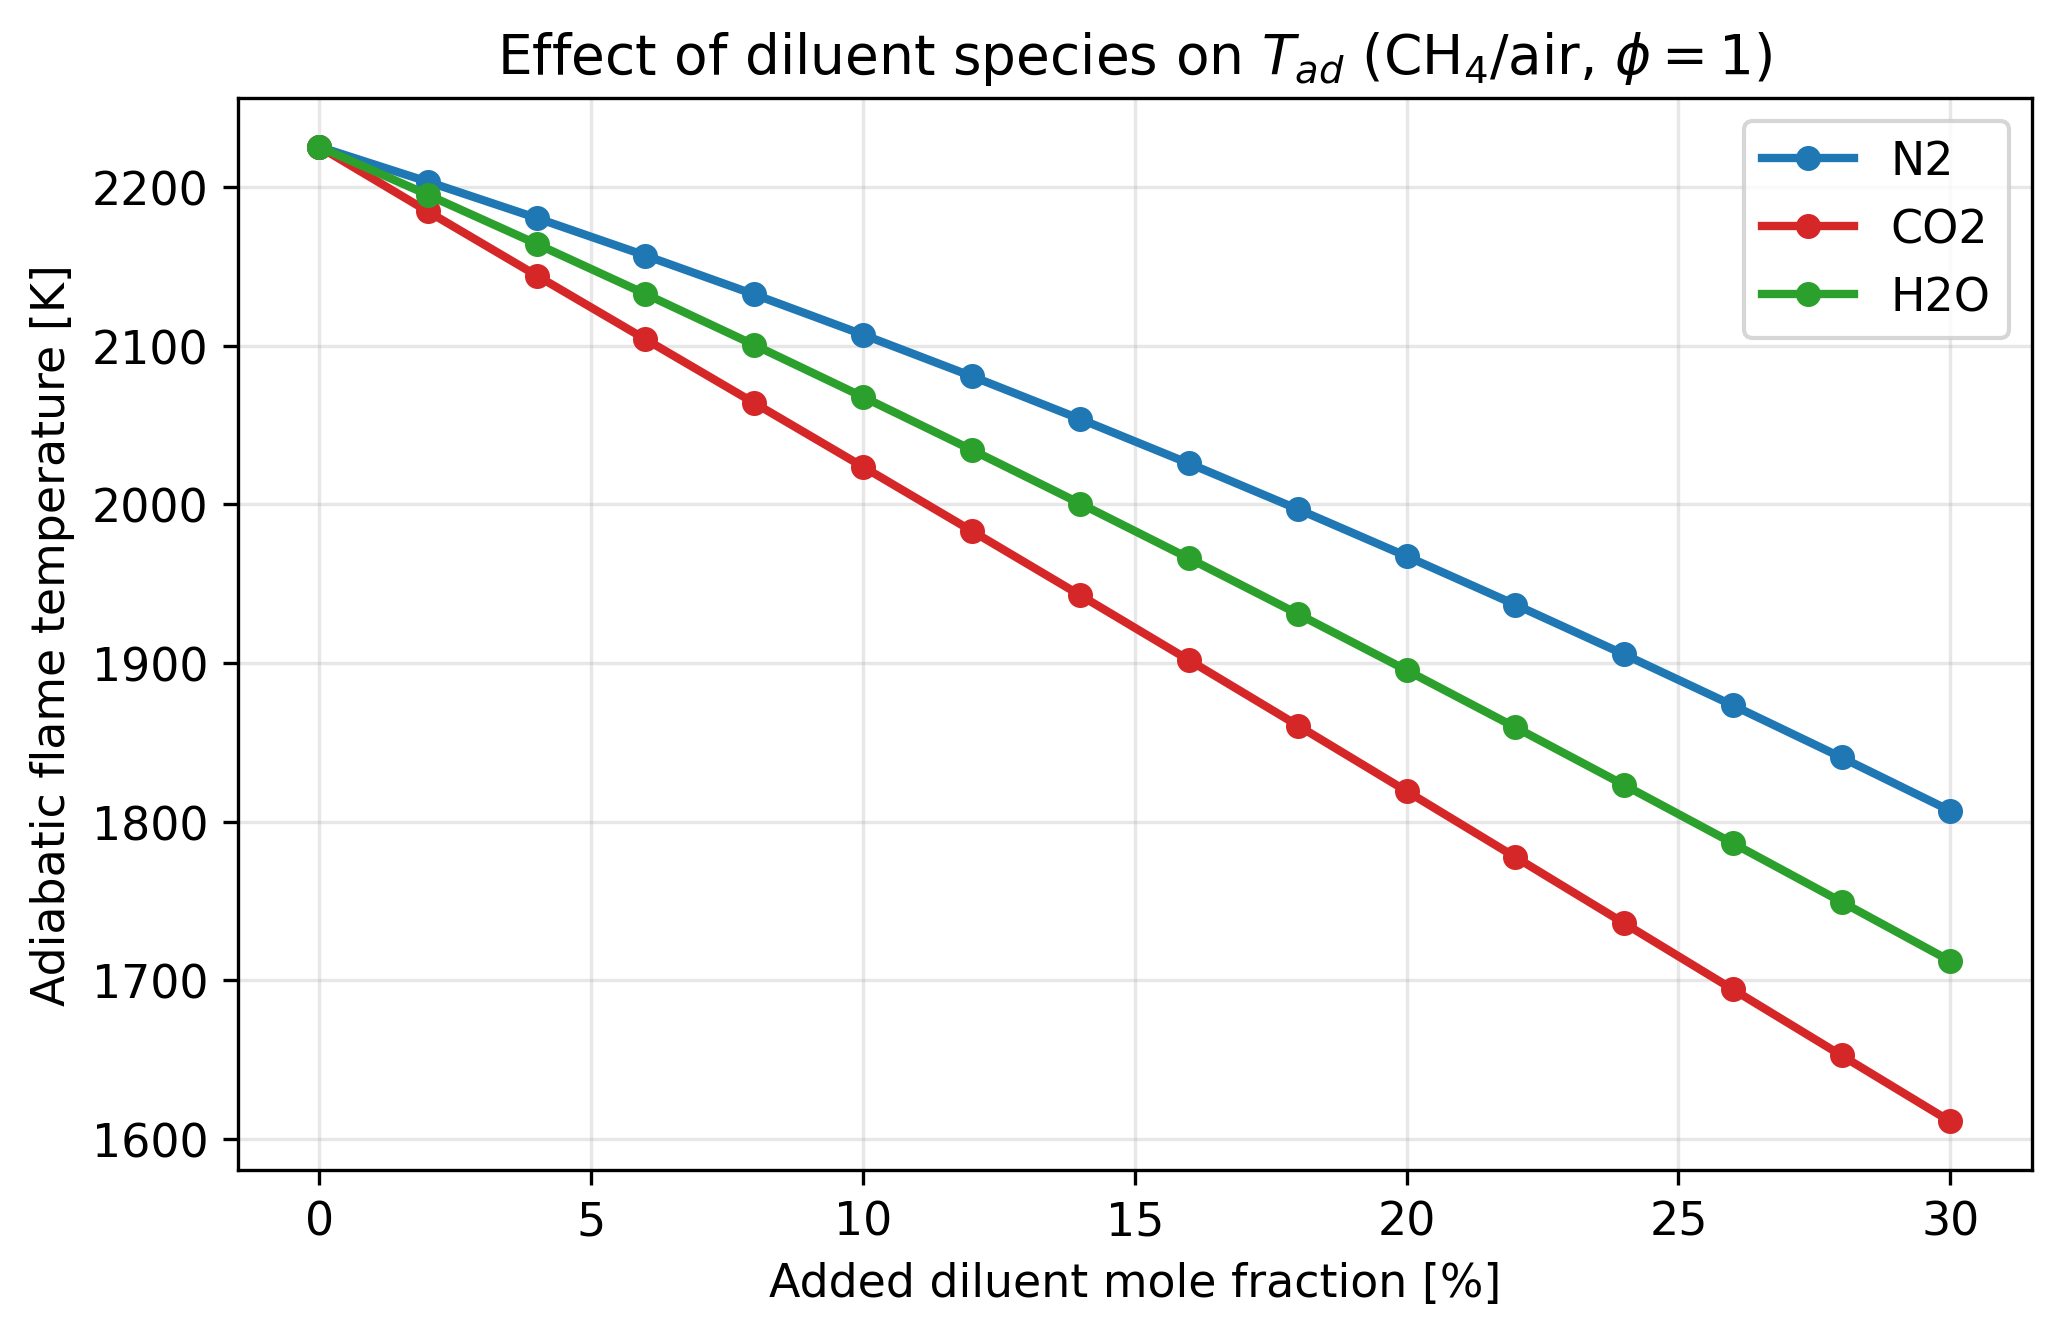
\includegraphics[width=\linewidth]{fig1_tad_vs_diluent.png}
    \caption{Effect of diluent species.}
    \label{fig:tad_dil}
  \end{subfigure}\hfill
  \begin{subfigure}{0.49\textwidth}
    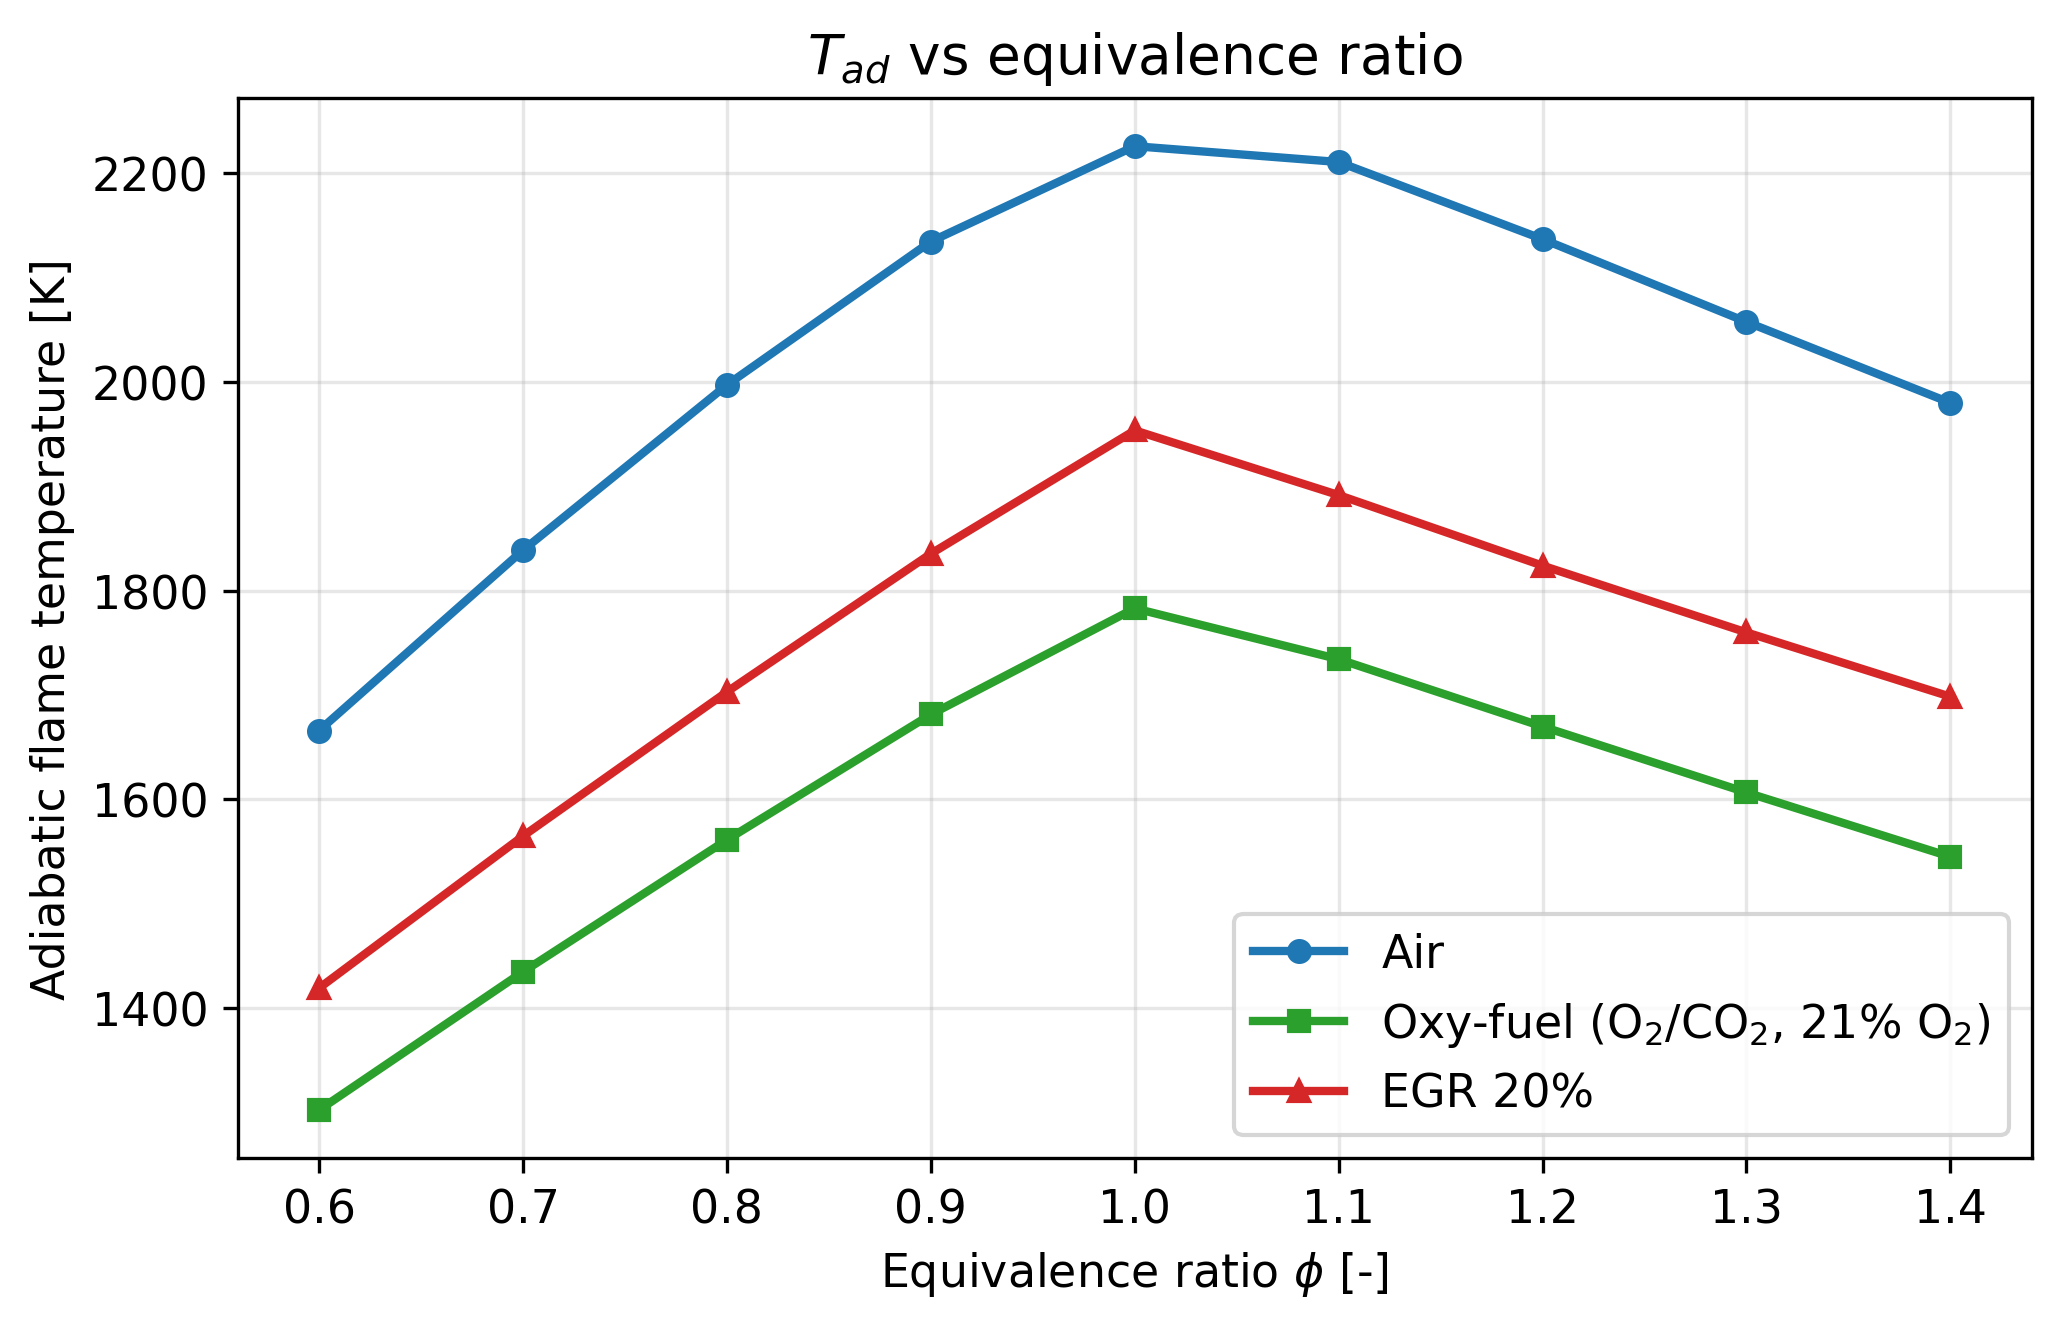
\includegraphics[width=\linewidth]{fig2_tad_vs_phi.png}
    \caption{Air vs.\ oxy-fuel vs.\ EGR.}
    \label{fig:tad_phi}
  \end{subfigure}
  \caption{Adiabatic flame temperature. Left: pure-diluent study at $\phi=1$.
  Right: the three combustion regimes across the equivalence-ratio range.}
  \label{fig:tad}
\end{figure}

Figure~\ref{fig:tad_phi} compares the three regimes across $\phi$. All curves
peak slightly rich, near $\phi \approx 1.0$--$1.05$. At stoichiometry the air
flame reaches 2225 K; 20 \% EGR lowers this to
1957 K, and oxy-fuel at $x_{\mathrm{O_2}} = 0.21$ falls to only
1783 K. The oxy-fuel case is the coldest precisely because its bath
gas is entirely CO\textsubscript{2}; in practice oxy-fuel combustors run with
$x_{\mathrm{O_2}}$ well above 21 \% to recover flame temperature, as
quantified below.

\subsection{Laminar flame speed}
Figure~\ref{fig:sl_phi} shows the laminar flame speed against equivalence ratio.
The air baseline peaks at 39 cm/s near $\phi=1$, in good
agreement with accepted data. 10 \% EGR cuts the peak to about
27 cm/s, and CO\textsubscript{2}-diluted oxy-fuel at
$x_{\mathrm{O_2}}=0.30$ to about 18 cm/s. The colder,
diluted flames are uniformly slower, which in a real combustor narrows the
stable operating window and raises the risk of blow-off.

\begin{figure}[H]
  \centering
  \begin{subfigure}{0.49\textwidth}
    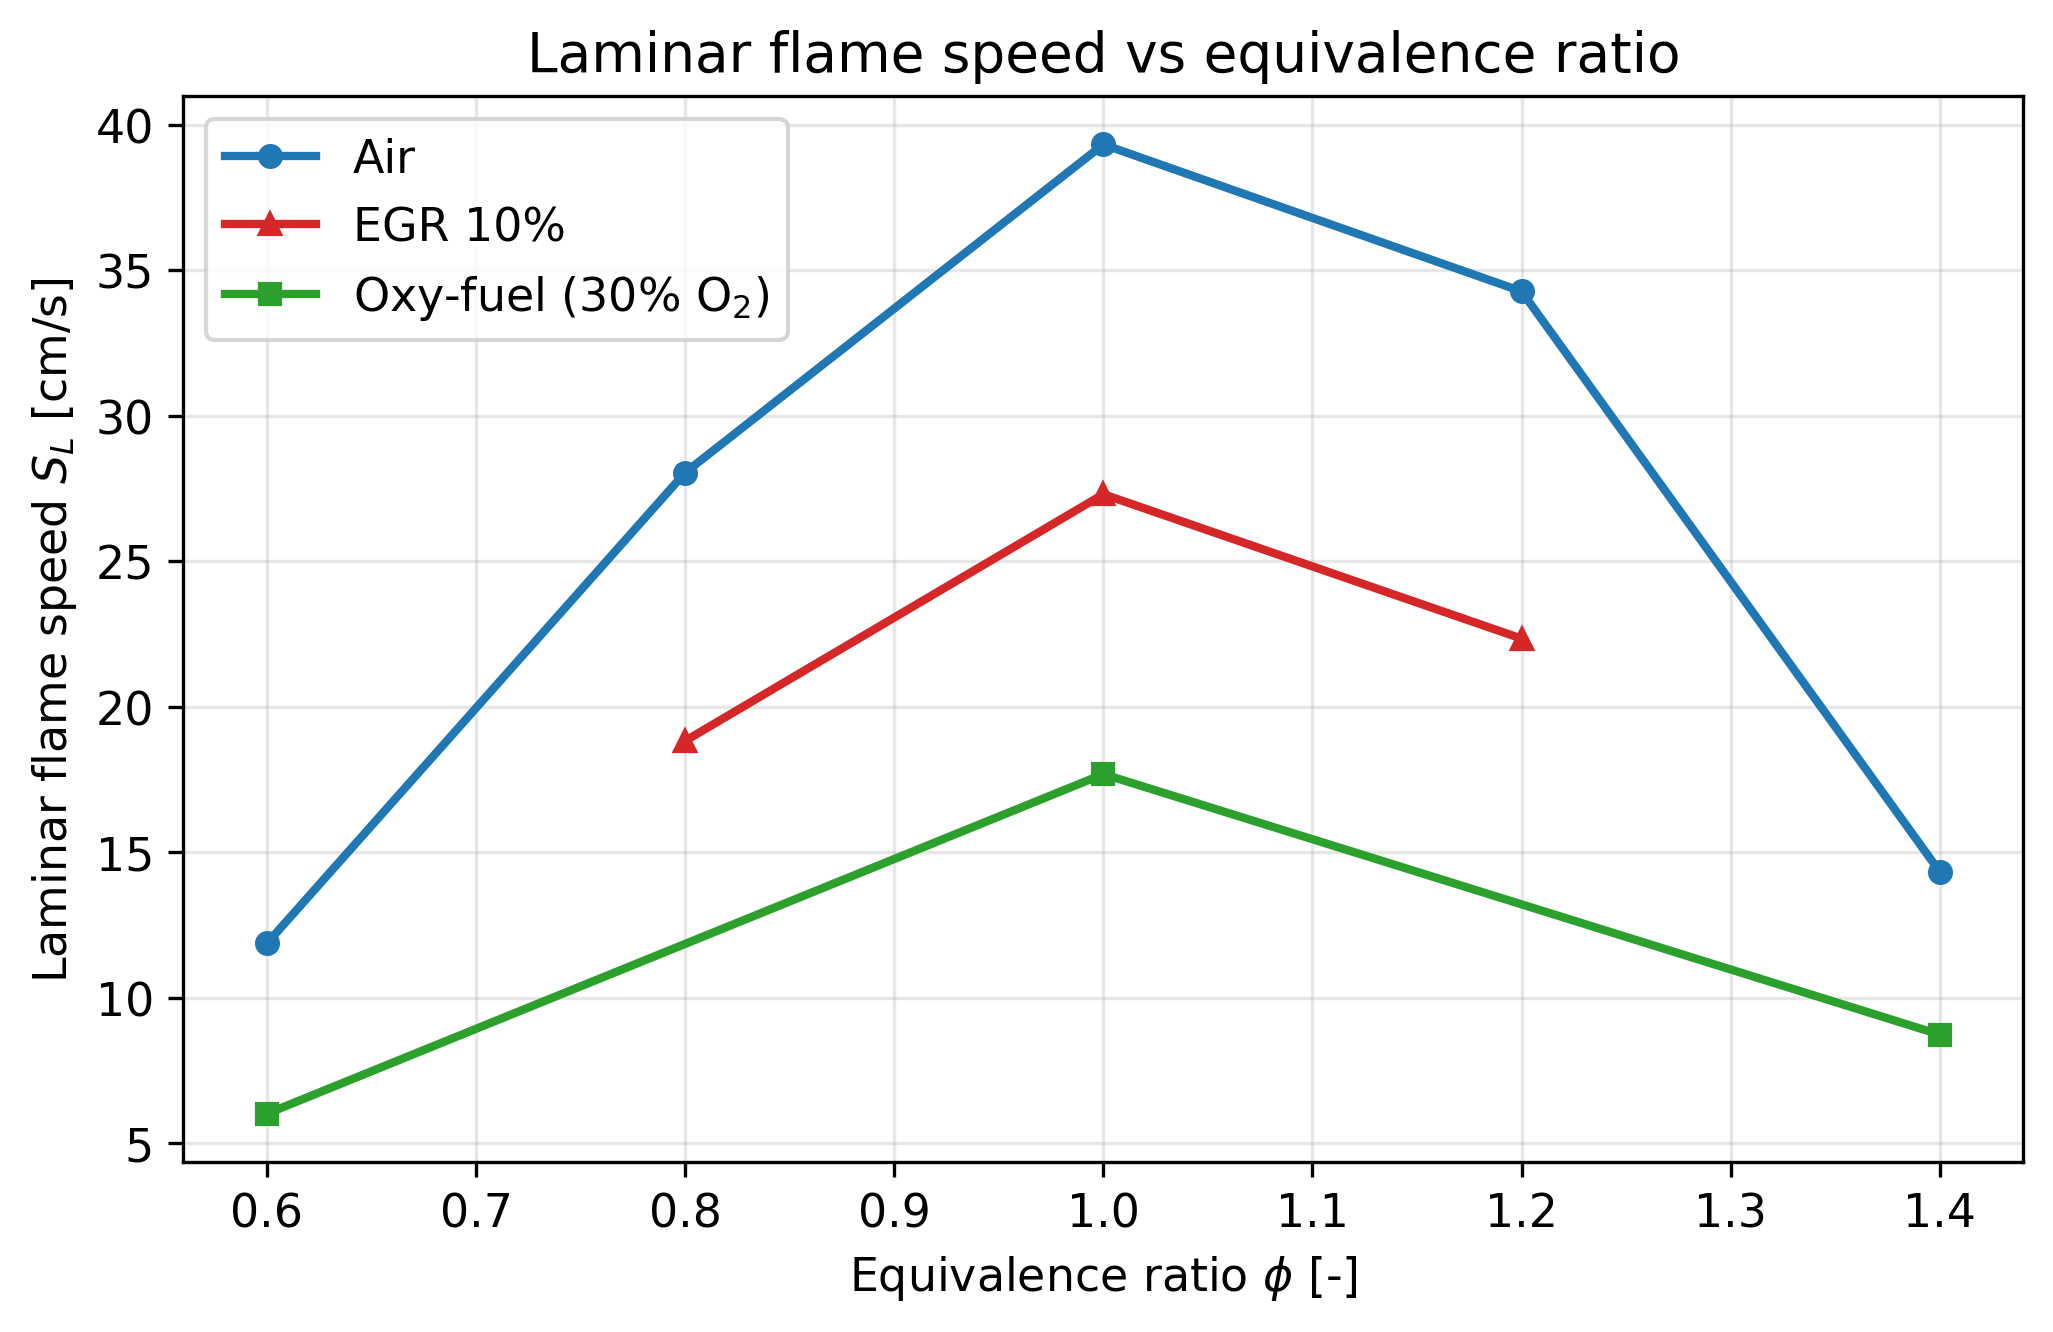
\includegraphics[width=\linewidth]{fig3_flamespeed_vs_phi.png}
    \caption{Flame speed vs.\ equivalence ratio.}
    \label{fig:sl_phi}
  \end{subfigure}\hfill
  \begin{subfigure}{0.49\textwidth}
    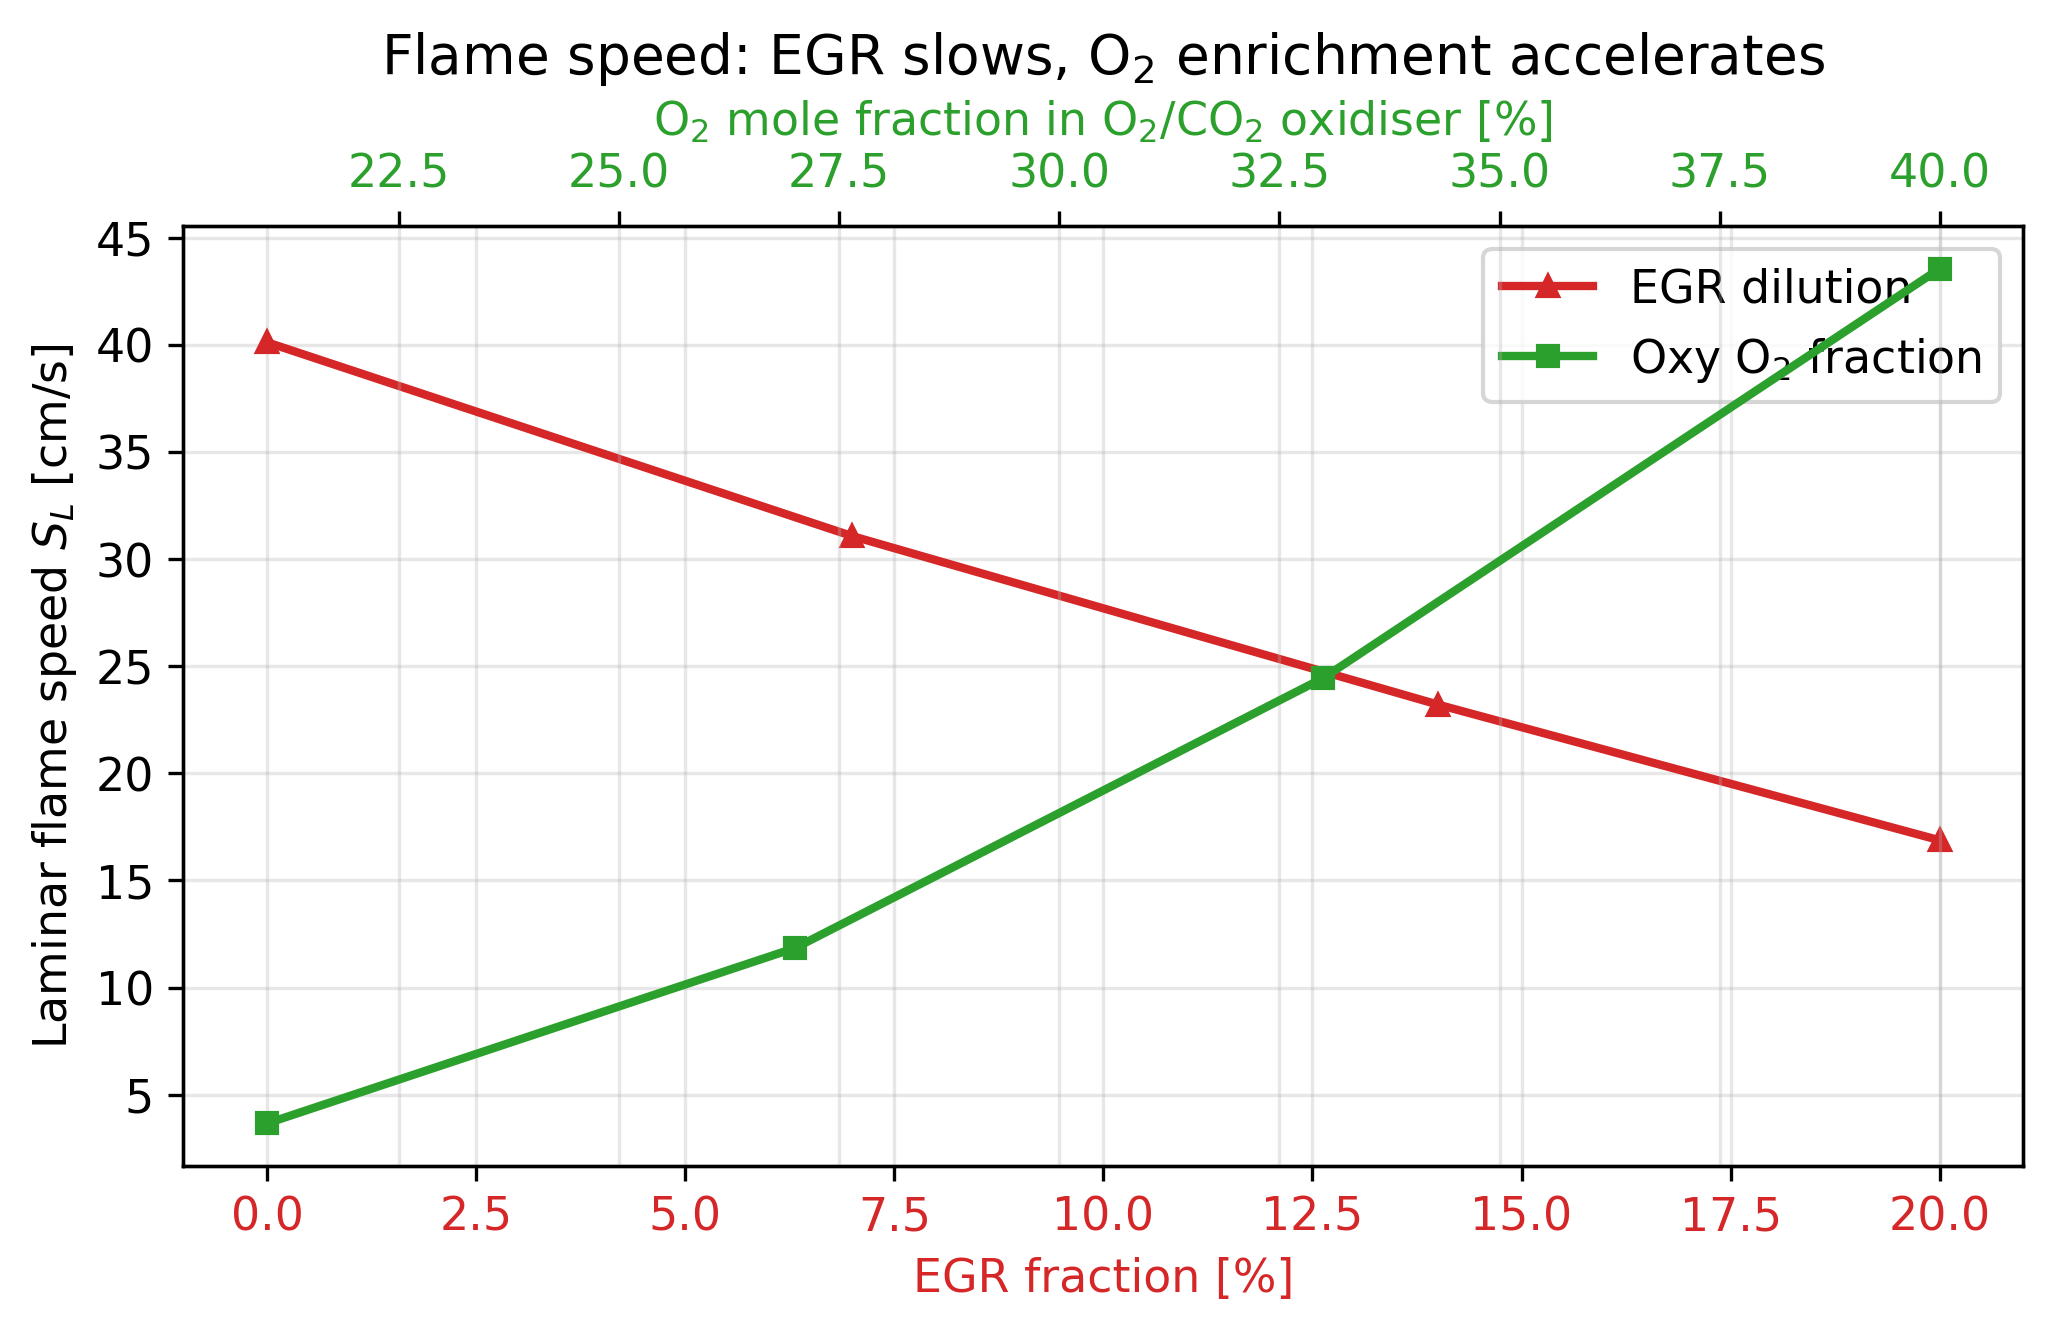
\includegraphics[width=\linewidth]{fig4_flamespeed_vs_dilution.png}
    \caption{Dilution and O\textsubscript{2}-enrichment sweeps.}
    \label{fig:sl_dil}
  \end{subfigure}
  \caption{Laminar flame speed. Right: at $\phi=1$, EGR monotonically slows the
  flame, whereas raising the O\textsubscript{2} fraction of the
  O\textsubscript{2}/CO\textsubscript{2} oxidiser accelerates it.}
  \label{fig:sl}
\end{figure}

Figure~\ref{fig:sl_dil} sweeps the two dilution parameters at stoichiometry.
Increasing EGR from 0 to 20 \% drops $S_L$ from 40 to
17 cm/s. Conversely, raising the oxygen fraction of the
O\textsubscript{2}/CO\textsubscript{2} oxidiser from 0.21 to 0.40
lifts $S_L$ from a sluggish 3.7 to 44 cm/s ---
above the air value --- which is exactly the lever used to restore flame speed
and stability in practical oxy-fuel systems.

\subsection{Auto-ignition delay}
Figure~\ref{fig:ign_arr} presents the ignition delay on an Arrhenius axis. All
three regimes collapse onto a nearly straight line spanning four orders of
magnitude between 1800 K ($\tau \approx 30 $\mu$s$) and
1000 K ($\tau \approx 0.18 s$ for air). Dilution has only
a modest kinetic effect at fixed temperature, but because EGR also lowers the
charge reactivity, the EGR curve sits at the longest delays on the cold
(right-hand) side of the plot.

\begin{figure}[H]
  \centering
  \begin{subfigure}{0.49\textwidth}
    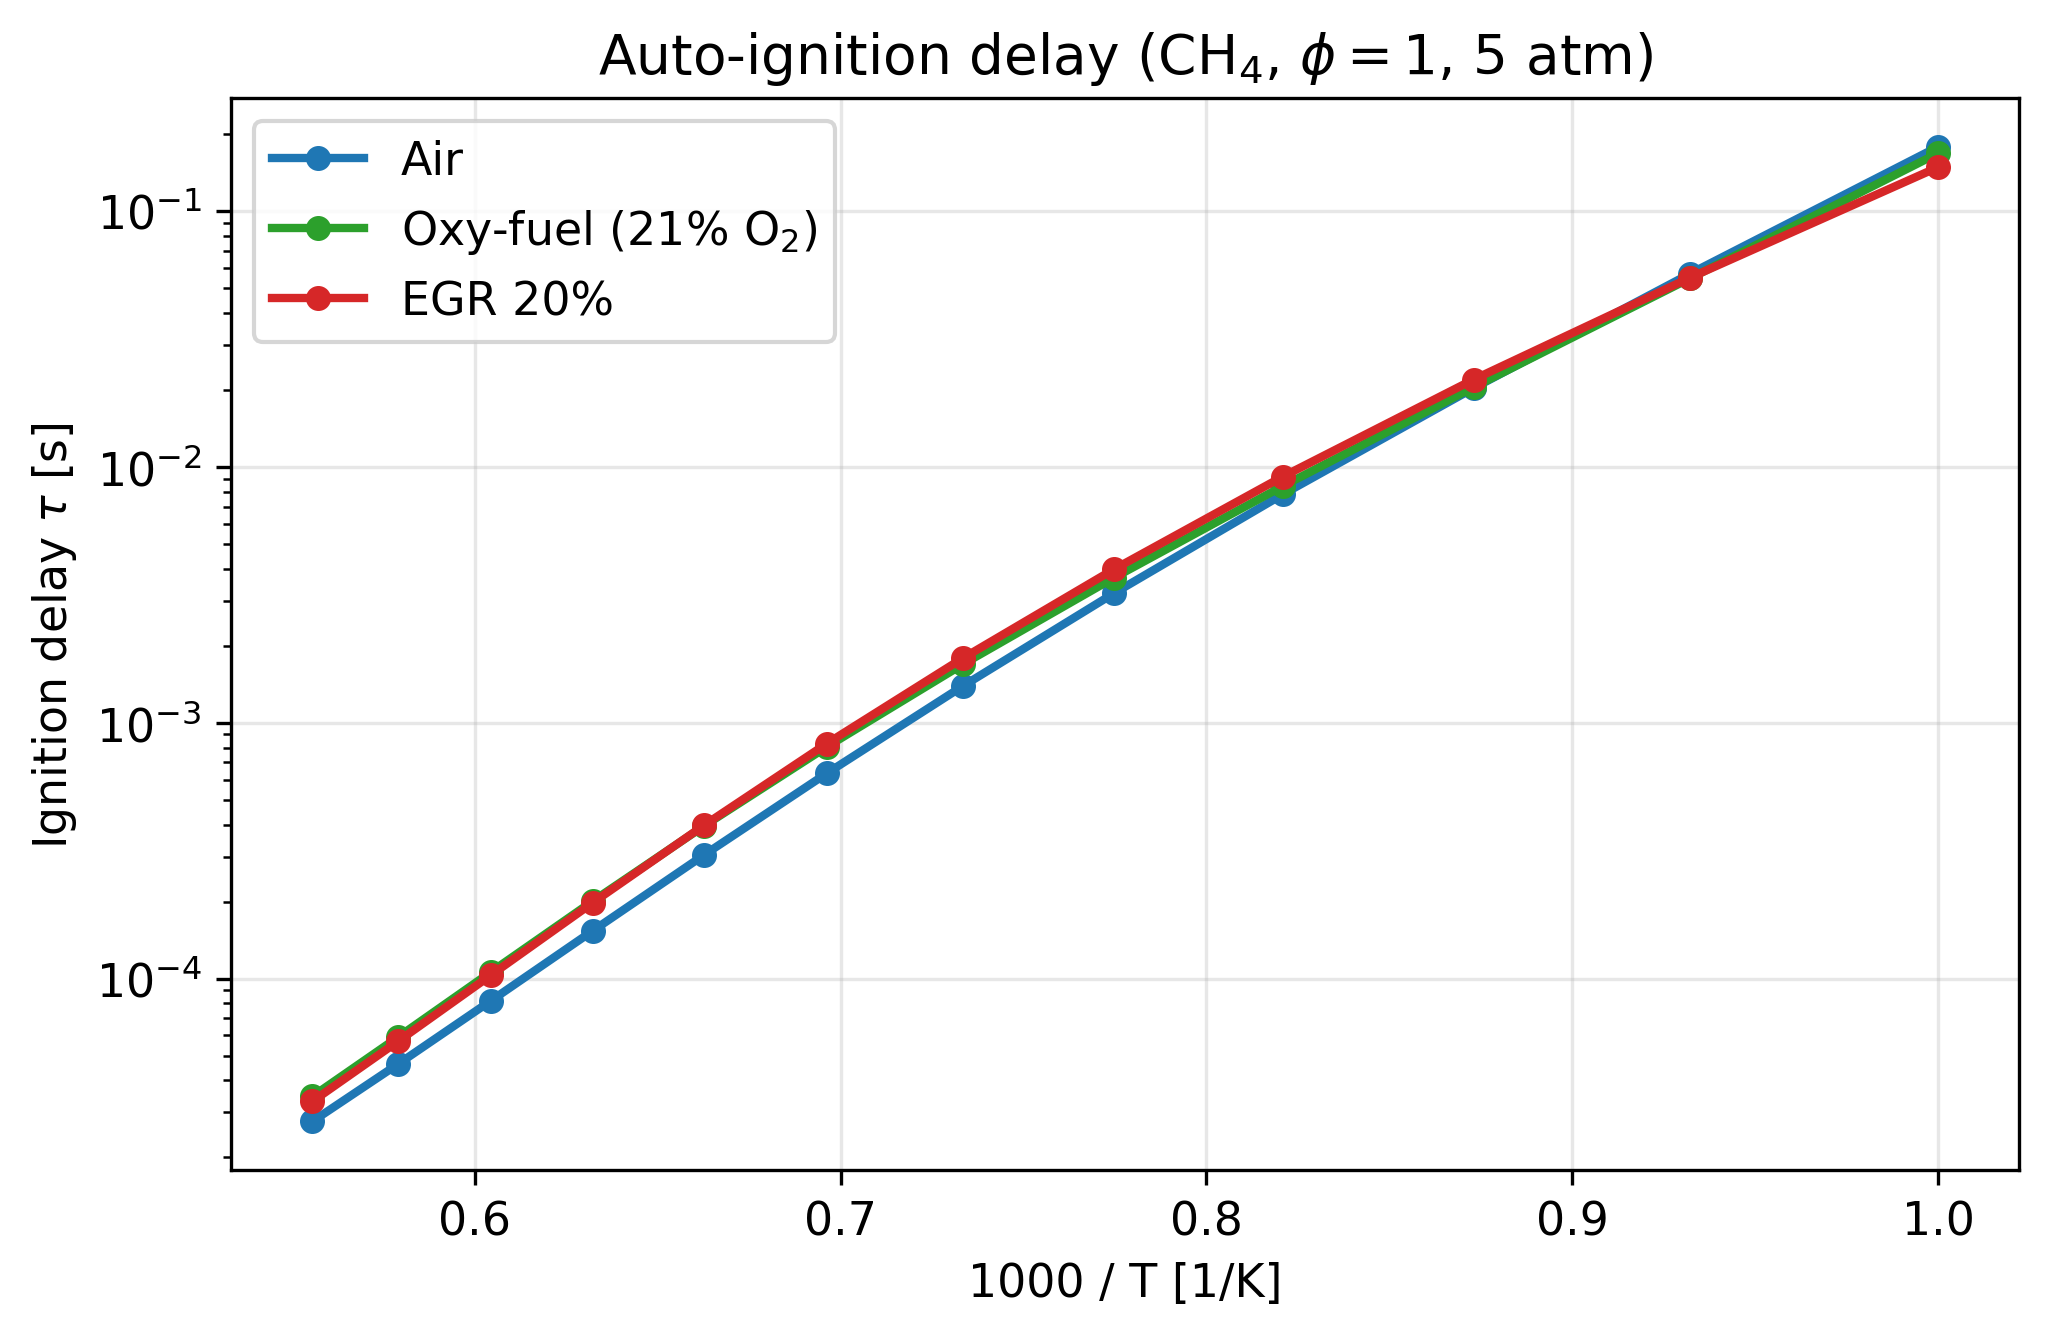
\includegraphics[width=\linewidth]{fig5_ignition_arrhenius.png}
    \caption{Arrhenius plot, $\phi=1$, 5 atm.}
    \label{fig:ign_arr}
  \end{subfigure}\hfill
  \begin{subfigure}{0.49\textwidth}
    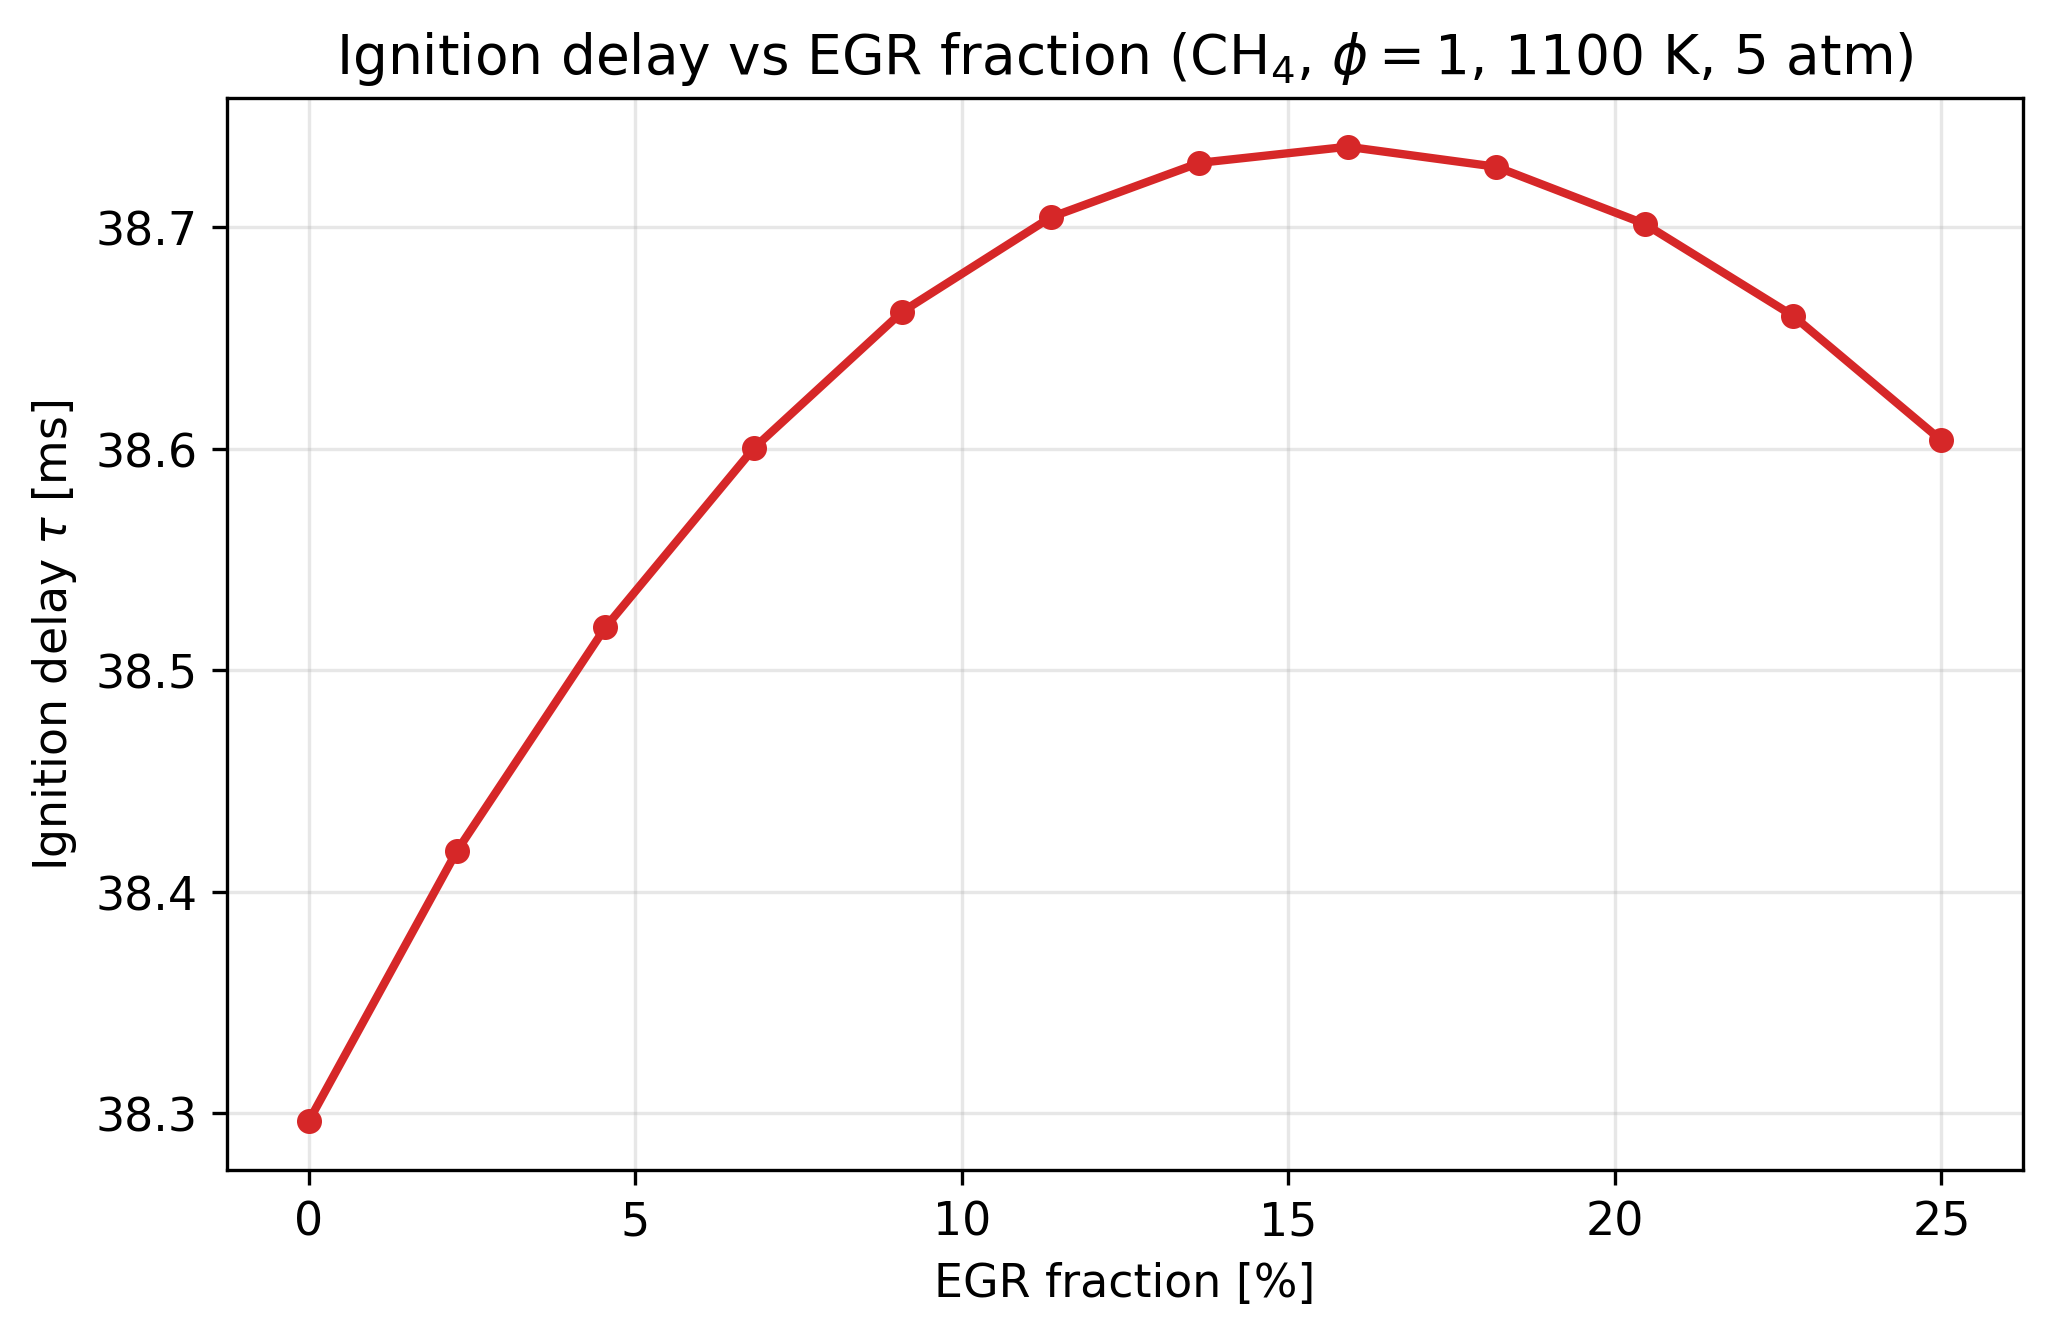
\includegraphics[width=\linewidth]{fig6_ignition_vs_egr.png}
    \caption{Ignition delay vs.\ EGR fraction.}
    \label{fig:ign_egr}
  \end{subfigure}
  \caption{Auto-ignition delay in a constant-pressure reactor. EGR lengthens the
  delay roughly linearly with the recirculated fraction.}
  \label{fig:ign}
\end{figure}

Figure~\ref{fig:ign_egr} isolates the EGR effect at a fixed 1100 K:
the delay grows roughly linearly with the recirculated fraction, doubling by
about 25 \% EGR. This lengthening is the kinetic signature of charge
dilution and is one of the practical limits on how much EGR an engine can
tolerate before misfire.

\subsection{Pressure dependence of ignition}
Figure~\ref{fig:ignp} sweeps the initial pressure at a fixed 1100~K. The ignition
delay follows a clean power law $\tau \propto p^{-1.09}$ across the 1--40~atm
range, close to the inverse-first-order behaviour expected when the
rate-controlling chain chemistry is dominated by bimolecular reactions. Higher
pressure shortens the delay sharply, which is why the engine-relevant ignition
study was carried out at 5~atm rather than at atmospheric pressure.

\begin{figure}[H]
  \centering
  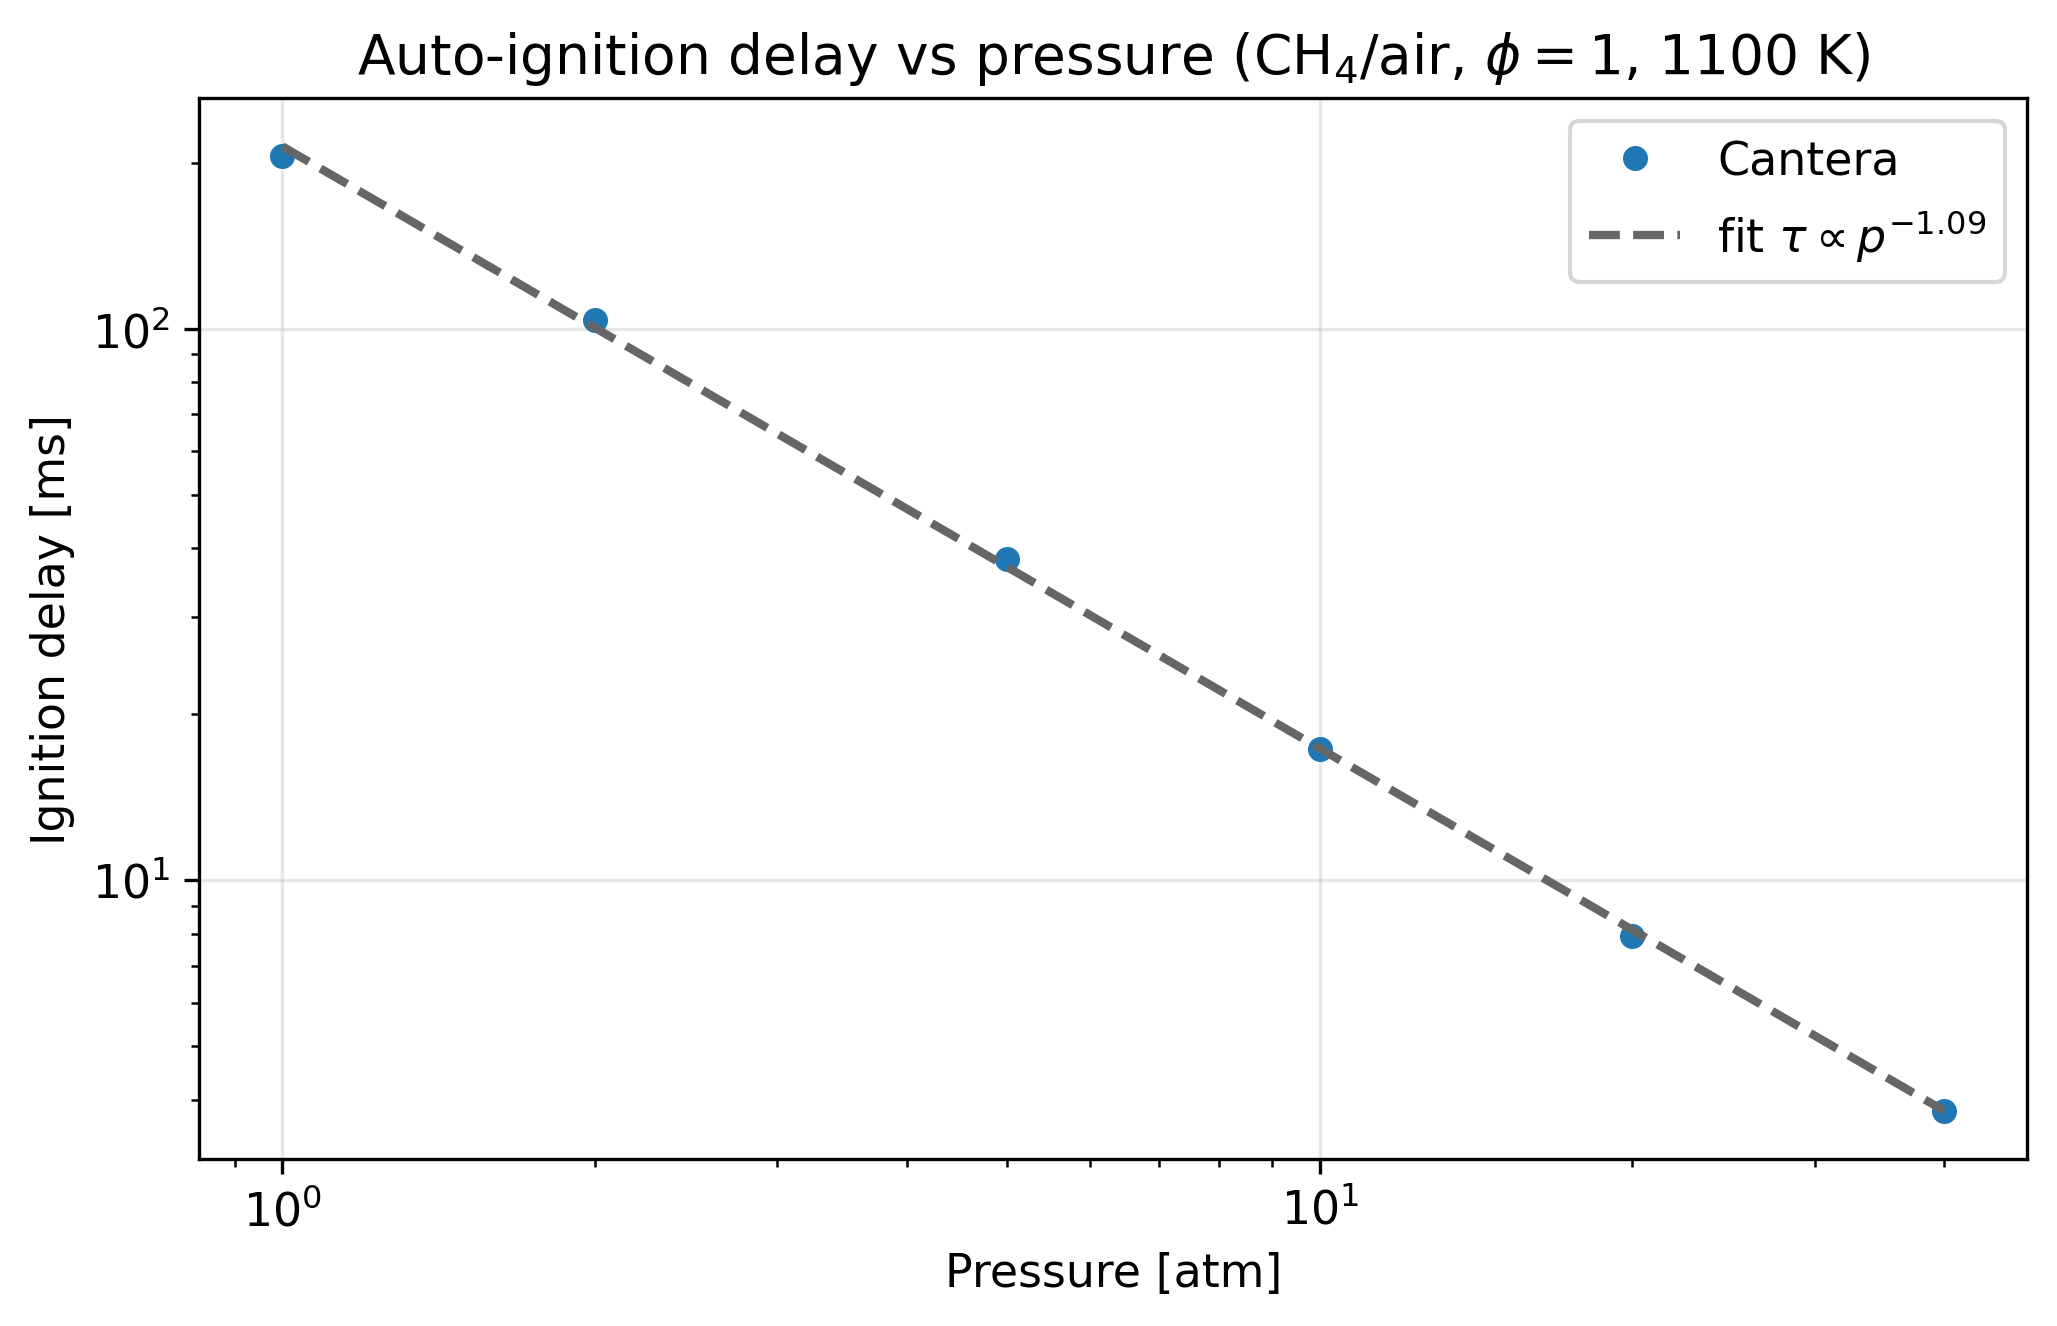
\includegraphics[width=0.62\textwidth]{fig10_ignition_vs_pressure.png}
  \caption{Auto-ignition delay versus pressure with a fitted power law.}
  \label{fig:ignp}
\end{figure}

\subsection{NO\texorpdfstring{\textsubscript{x}}{x} formation}
The emission payoff is summarised in Figures~\ref{fig:nox_phi}
and~\ref{fig:nox_egr}. For air, equilibrium NO peaks at roughly
3080 ppm slightly lean ($\phi \approx 0.85$), where temperature is still
high but oxygen is abundant --- the classic thermal-NO maximum.
20 \% EGR roughly halves the peak. Oxy-fuel combustion produces
essentially \emph{zero} NO across the whole range, simply because there is no
atmospheric nitrogen to oxidise.

\begin{figure}[H]
  \centering
  \begin{subfigure}{0.49\textwidth}
    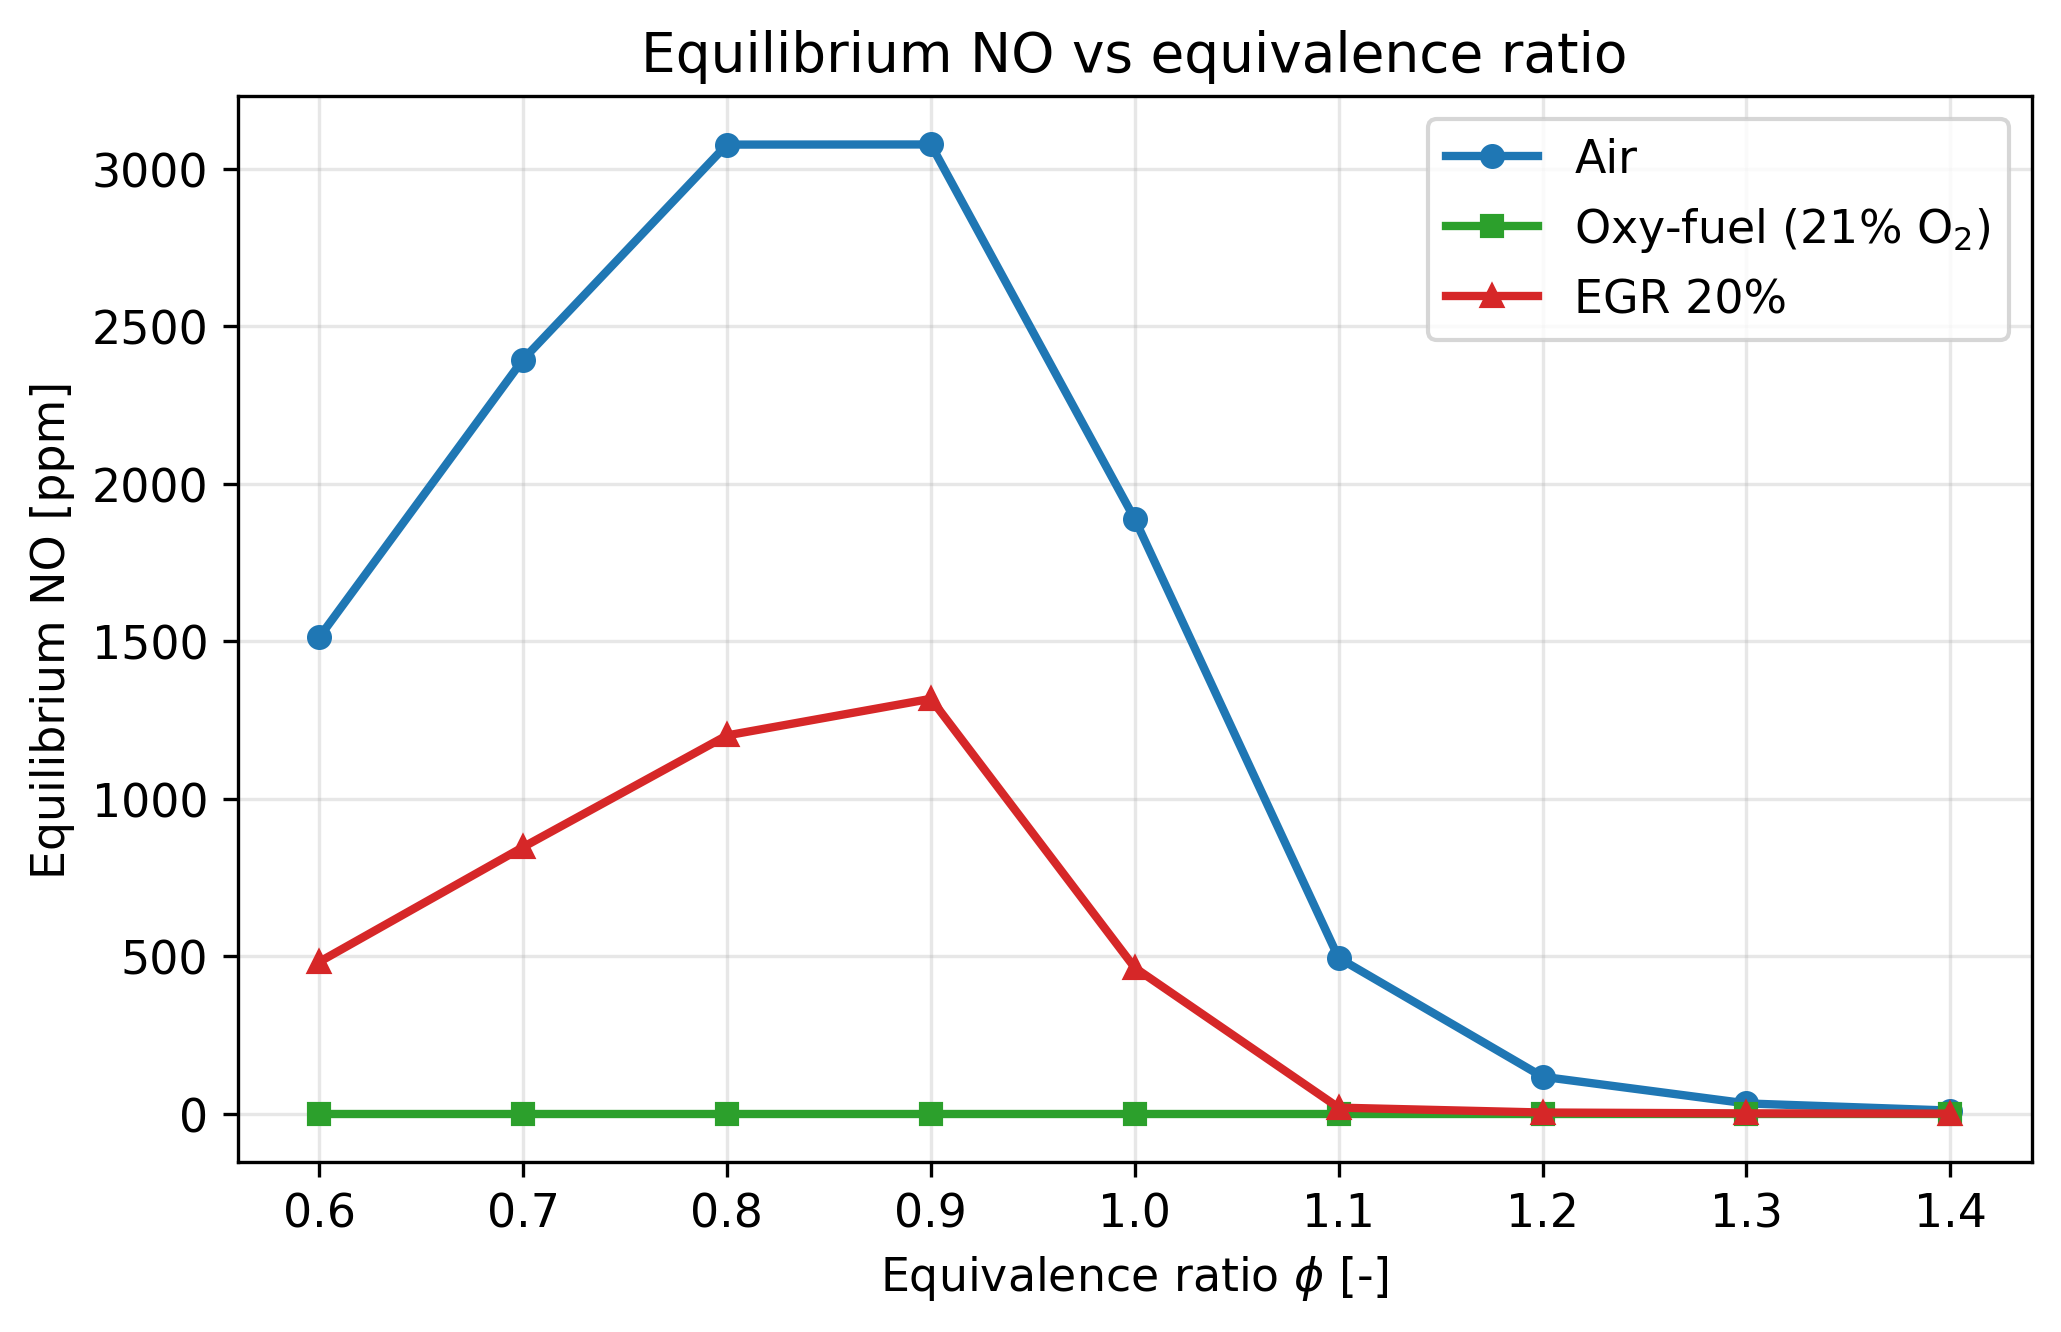
\includegraphics[width=\linewidth]{fig7_nox_vs_phi.png}
    \caption{Equilibrium NO vs.\ equivalence ratio.}
    \label{fig:nox_phi}
  \end{subfigure}\hfill
  \begin{subfigure}{0.49\textwidth}
    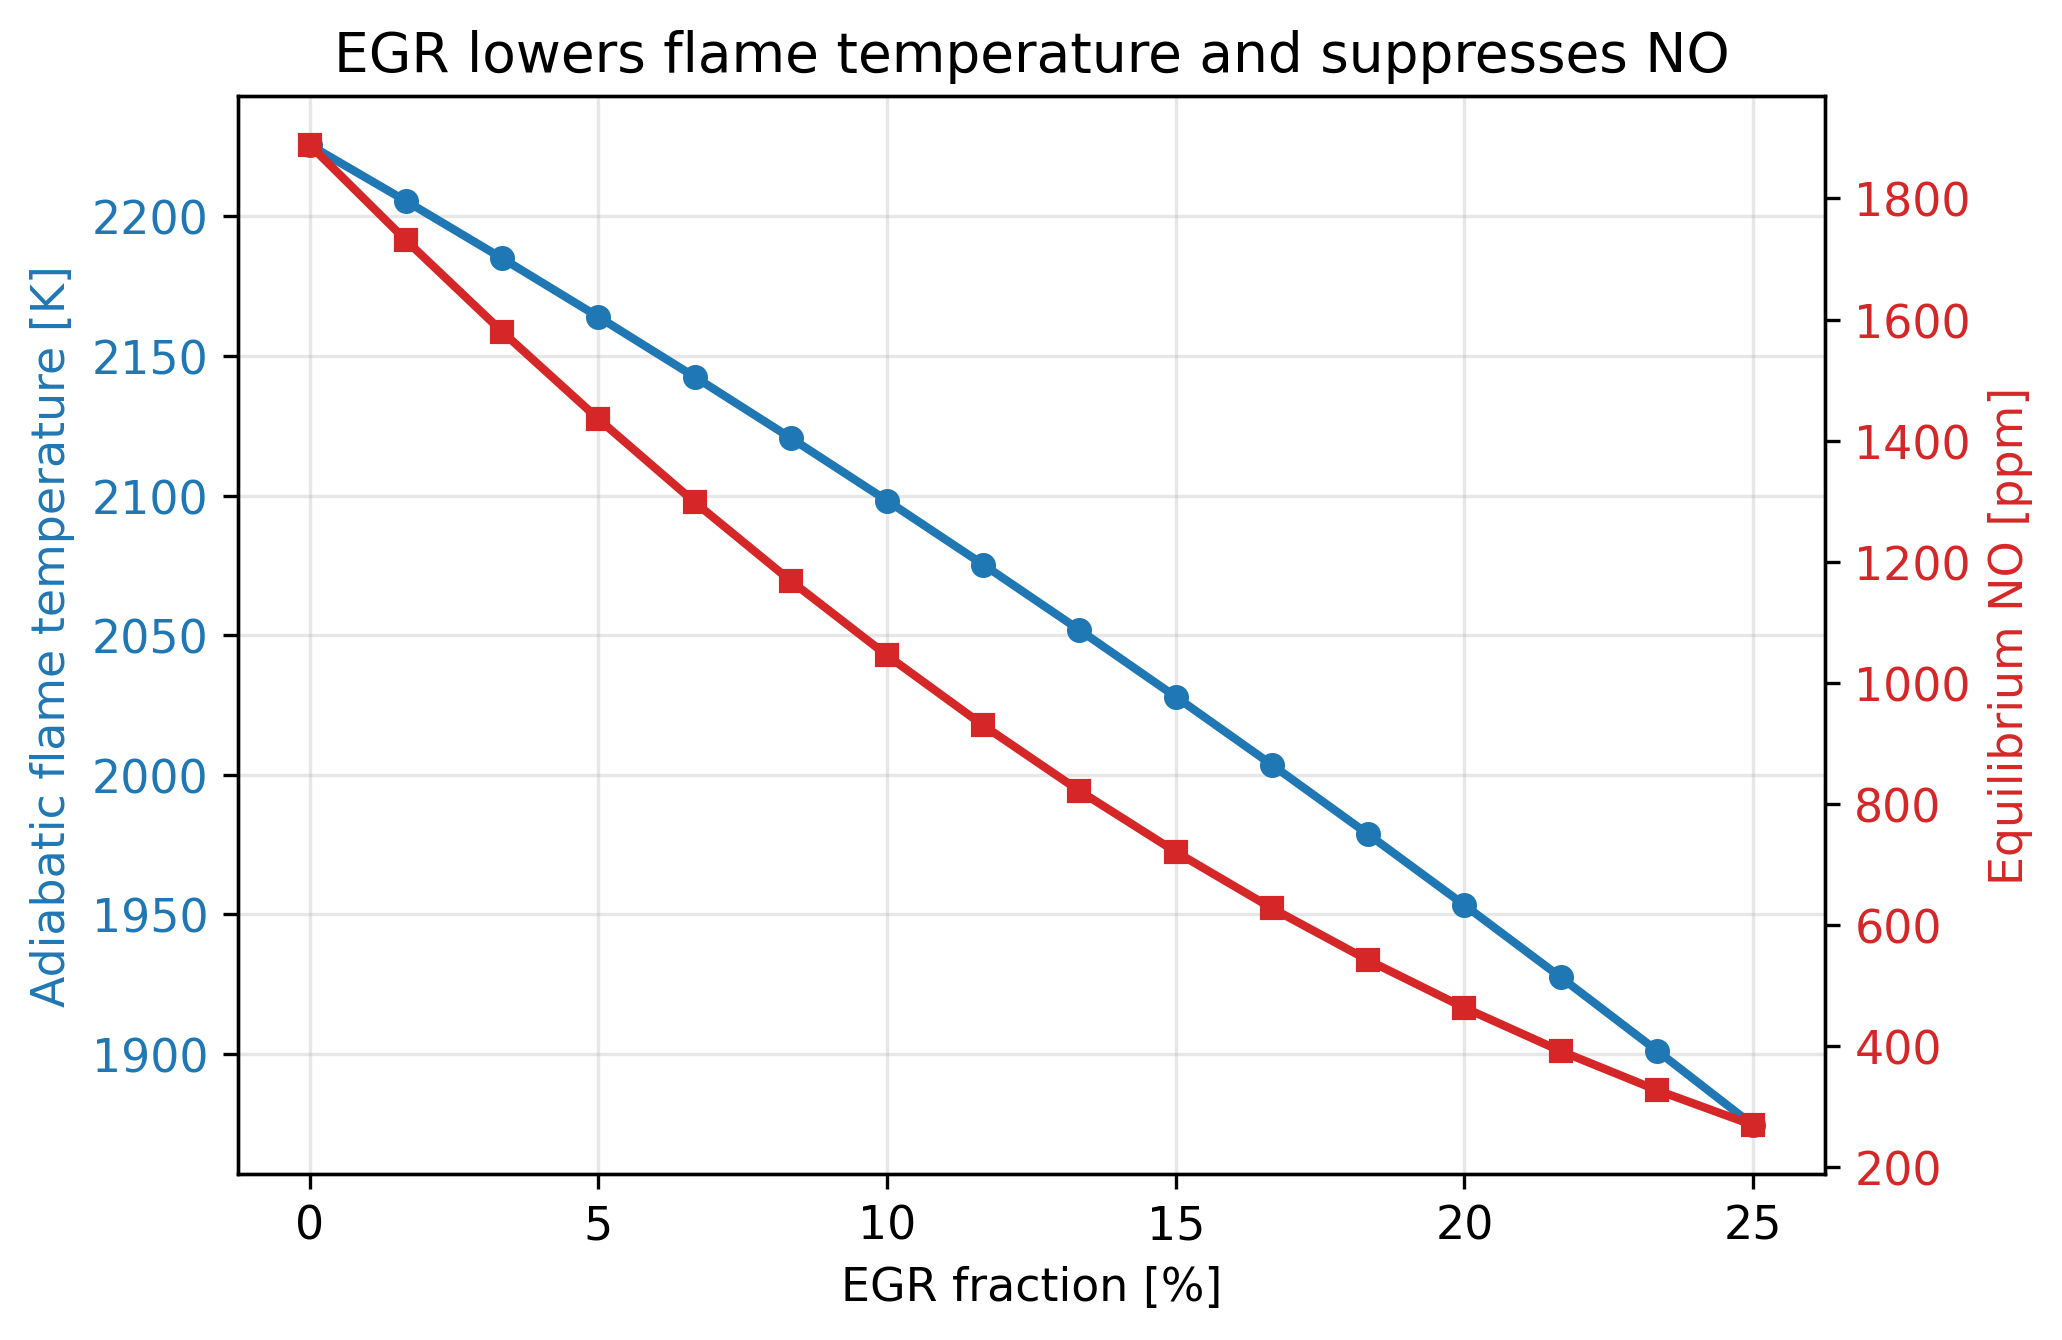
\includegraphics[width=\linewidth]{fig8_tad_no_vs_egr.png}
    \caption{NO and $T_{ad}$ vs.\ EGR fraction.}
    \label{fig:nox_egr}
  \end{subfigure}
  \caption{NO formation. The right-hand panel makes the EGR mechanism explicit:
  the NO reduction tracks the fall in flame temperature.}
  \label{fig:nox}
\end{figure}

Figure~\ref{fig:nox_egr} exposes the mechanism directly. As EGR rises from
0 to 25 \%, the stoichiometric flame temperature falls from
2225 to 1880 K and equilibrium NO collapses from about
1890 to 380 ppm --- a five-fold reduction driven almost entirely by
the temperature drop, since thermal NO is exponentially sensitive to $T$. This
single figure captures the central trade-off of low-emission combustion: NO is
bought down with flame temperature, and flame temperature is paid for in flame
speed and ignitability.

\subsection{Finite-rate NO kinetics}
The equilibrium NO above is an upper bound. Figure~\ref{fig:nokin} shows the
\emph{kinetic} build-up of NO, obtained by integrating the full mechanism at the
flame temperature with the nitrogen-oxide pool initially set to zero. Two effects
combine. First, thermal NO forms slowly: even the hot air flame needs tens of
milliseconds to approach its equilibrium value, so the NO actually emitted is
set by the residence time. Second, and more decisive for design, the lower flame
temperatures of EGR and oxy-fuel throttle the formation rate exponentially
through the Arrhenius dependence of the Zeldovich mechanism --- at 20\% EGR the
NO is still below 50~ppm after 0.5~s, two orders of magnitude
under the air value, and oxy-fuel produces essentially none. The kinetic picture
therefore reinforces the equilibrium result: dilution suppresses NO both
thermodynamically and kinetically.

\begin{figure}[H]
  \centering
  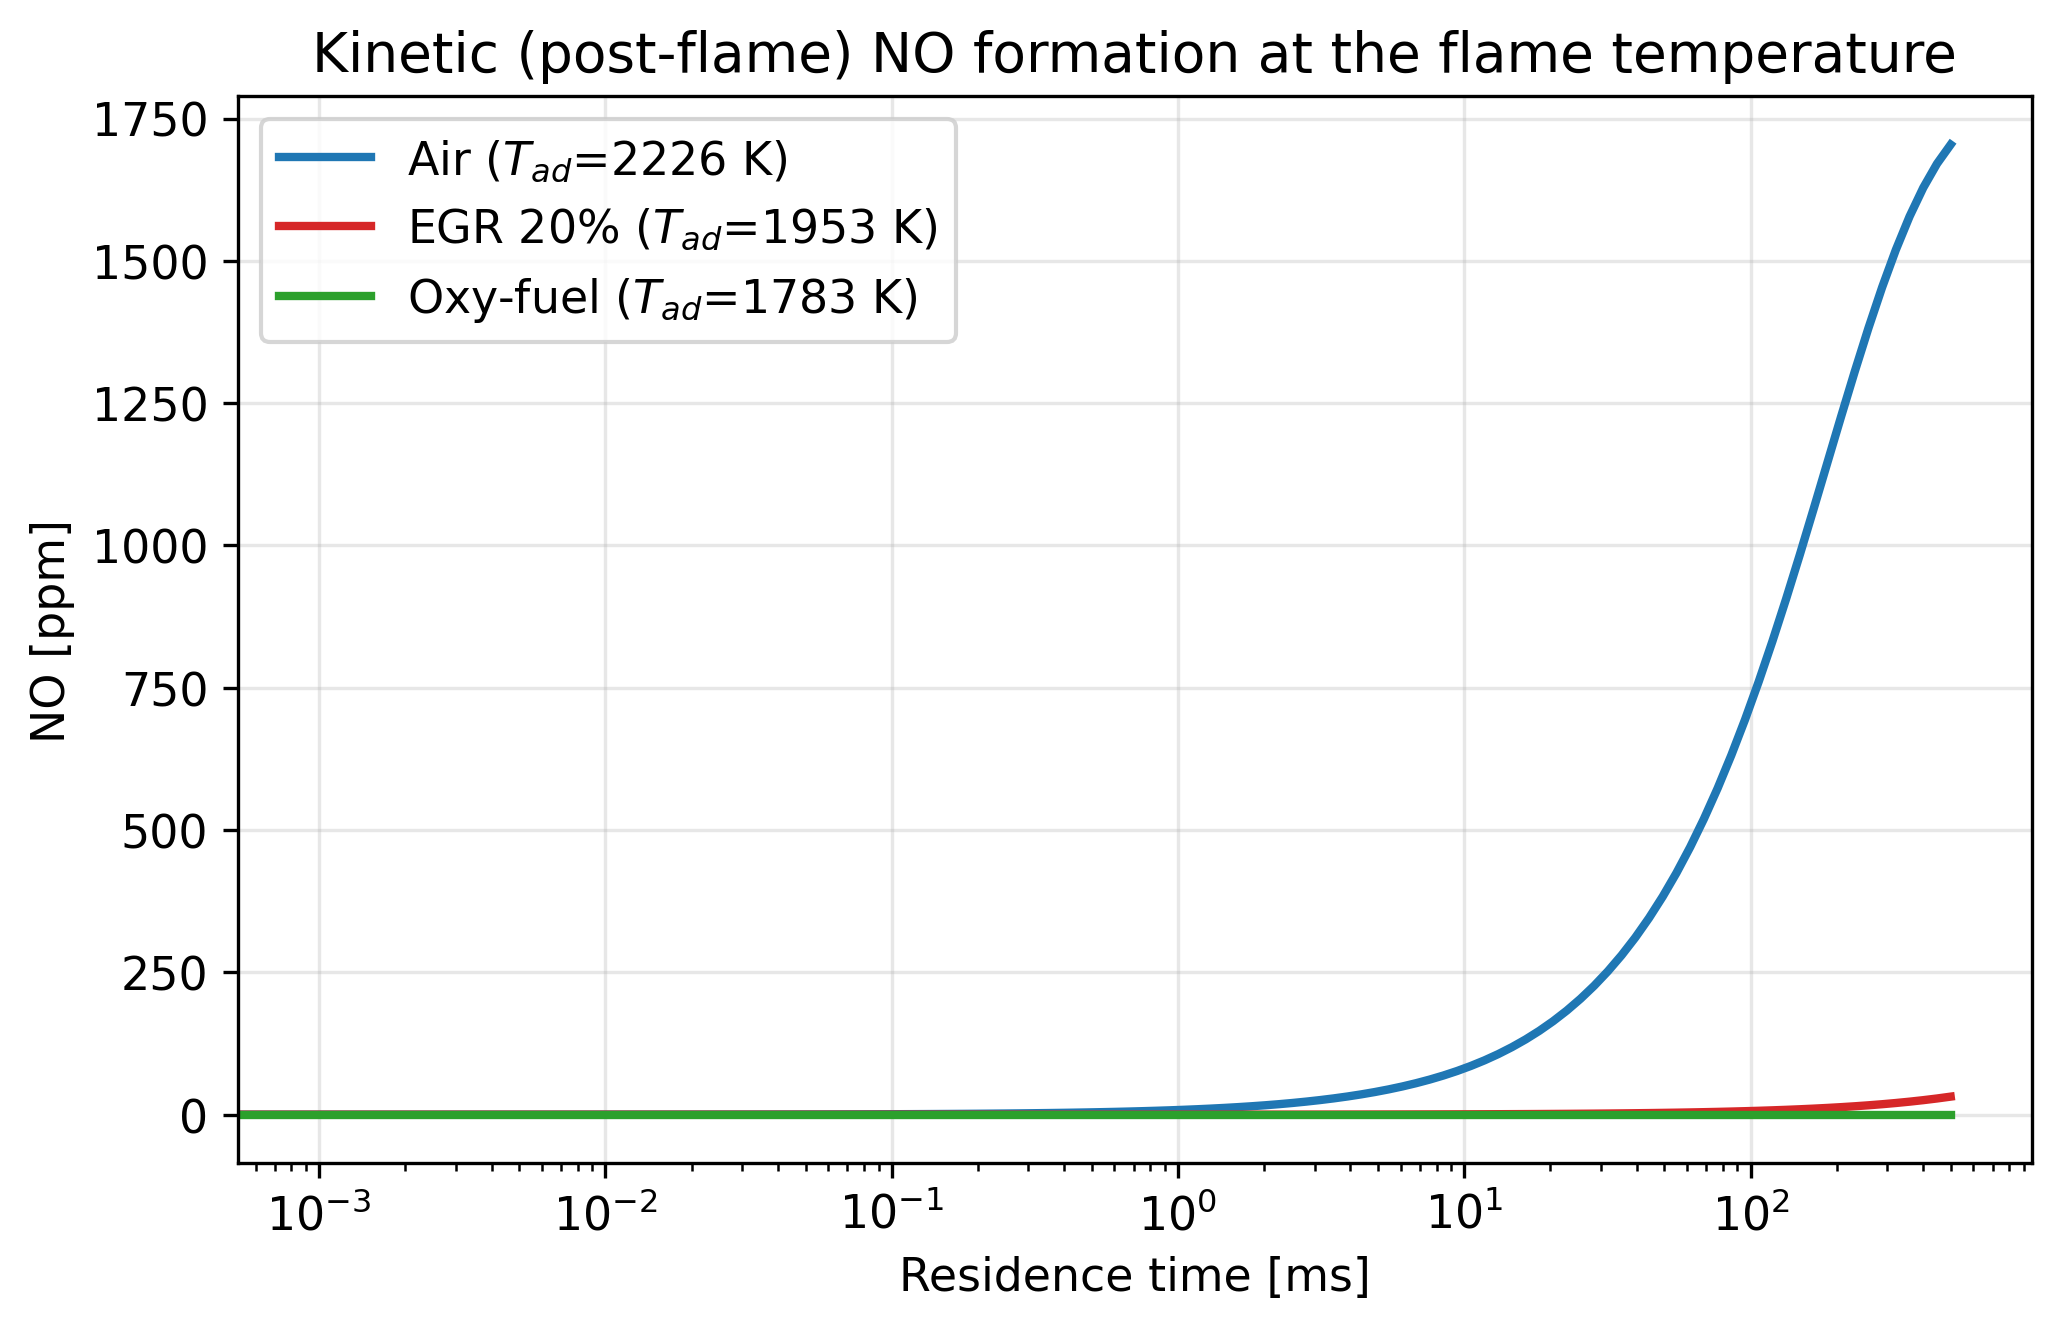
\includegraphics[width=0.66\textwidth]{fig9_no_kinetics.png}
  \caption{Kinetic (post-flame) NO formation at the flame temperature. Lower
  temperatures suppress NO not only at equilibrium but also kinetically.}
  \label{fig:nokin}
\end{figure}

\section{Conclusions}
A consistent \textsc{Cantera}/GRI-Mech~3.0 framework was used to compare
conventional, EGR-diluted and oxy-fuel methane combustion across four physically
distinct quantities. The main findings are:
\begin{enumerate}
  \item Both EGR and CO\textsubscript{2}-rich oxy-fuel operation lower the
  adiabatic flame temperature, CO\textsubscript{2} being a stronger diluent than
  N\textsubscript{2} per unit mole.
  \item The colder mixtures burn more slowly: 20 \% EGR more than
  halves the laminar flame speed, while increasing the oxygen fraction of an
  O\textsubscript{2}/CO\textsubscript{2} oxidiser is an effective way to recover
  --- and exceed --- the air flame speed.
  \item Auto-ignition follows Arrhenius behaviour over four decades; EGR lengthens
  the ignition delay roughly linearly, setting a practical dilution limit.
  \item Thermal NO falls steeply with flame temperature: EGR delivers a several-fold
  reduction, and oxy-fuel combustion eliminates thermal NO outright while
  yielding a capture-ready CO\textsubscript{2} exhaust. A finite-rate reactor
  confirms that dilution suppresses NO kinetically as well as thermodynamically,
  and that the emitted NO is residence-time limited.
  \item Auto-ignition delay obeys a power law $\tau \propto p^{-1.09}$ in
  pressure, so engine-pressure operation ignites far faster than the
  atmospheric-pressure case.
\end{enumerate}
Together the results quantify, in one place, the temperature--speed--ignition--
emission trade-off that underlies modern low-NO\textsubscript{x} and
carbon-capture-ready combustor design. NO was treated at both the equilibrium and
finite-rate levels; the remaining modelling limitations are the use of GRI-Mech
3.0 (validated for natural gas rather than for ammonia- or CO\textsubscript{2}-rich
oxy chemistry) and the single-reactor residence-time model. A dedicated oxy-fuel
mechanism and a networked reactor model would refine the absolute emission levels
without changing the qualitative conclusions.

\begin{thebibliography}{9}
\bibitem{cantera} D.~G. Goodwin et al., \emph{Cantera: An Object-oriented
Software Toolkit for Chemical Kinetics, Thermodynamics, and Transport
Processes}, version 3.2, 2024. \url{https://www.cantera.org}
\bibitem{gri} G.~P. Smith et al., \emph{GRI-Mech 3.0}, Gas Research Institute.
\url{http://combustion.berkeley.edu/gri-mech/}
\bibitem{law} C.~K. Law, \emph{Combustion Physics}, Cambridge University Press,
2006.
\bibitem{turns} S.~R. Turns, \emph{An Introduction to Combustion: Concepts and
Applications}, 3rd ed., McGraw-Hill, 2012.
\bibitem{oxy} B.~J.~P. Buhre et al., \emph{Oxy-fuel combustion technology for
coal-fired power generation}, Progress in Energy and Combustion Science, 31(4),
2005.
\end{thebibliography}

\end{document}
